\documentclass[12pt,a4paper]{article}
\usepackage[paper=portrait,pagesize]{typearea}
\usepackage[left=2cm, right=2cm]{geometry}
\usepackage[utf8]{inputenc}
\usepackage[hidelinks]{hyperref}
\usepackage{graphicx, indentfirst, array, lscape, caption, subcaption, minted}
\graphicspath{ {./images/} }

\renewcommand\contentsname{Índice}
\renewcommand\refname{Referências}
\renewcommand{\listfigurename}{Lista de Figuras}
\renewcommand{\figurename}{Figura}

\title{

\begin{figure}[t!]
    
\includegraphics[keepaspectratio, width=0.5\textwidth]{logoISEL}
\end{figure}

    \textbf{Licenciatura em Engenharia Informática e de Computadores} \vspace{5mm} \\
    \textbf{Queuality} \\ 
    \vspace{5mm}
    Sistema de Gestão de Filas de Espera
}
\author{
    Joana Campos, A44792 \href{mailto:a44792@alunos.isel.pt}{a44792@alunos.isel.pt} 
    \and Nuno Cardeal, A44863 \href{mailto:a44863@alunos.isel.pt}{a44863@alunos.isel.pt}
    \and Carolina Couto, A44871 \href{mailto:a44871@alunos.isel.pt}{a44871@alunos.isel.pt} \\
    \\
    \textbf{Orientador:} Paulo Pereira \href{mailto:paulo.pereira@isel.pt}{paulo.pereira@isel.pt}
}
\date{Junho 2021}
\begin{document}

\maketitle
\thispagestyle{empty}
\pagebreak
\pagenumbering{roman}
\tableofcontents
\pagebreak
\listoffigures
\pagebreak
\pagenumbering{arabic}


\pagebreak
\section{Introdução}
Numa sociedade onde existe cada vez mais adesão a \textit{multitasking}, estar preso numa fila de espera,
parado sem fazer nada, pode ser considerado uma perda de tempo. Tempo esse que poderia ser usado
para trabalhar ou para “ir beber um café”. Principalmente nestes tempos de pandemia estar em contacto
com outras pessoas deve ser evitado.\par

Para contornar esta situação, uma solução viável seria um sistema de gestão de filas de espera que,
assumindo que o cliente se encontra próximo do local onde espera ser servido, o notifica quando estiver
próximo da sua vez, evitando assim que o cliente tenha de estar presencialmente na fila, podendo ir
fazer outras coisas enquanto aguarda, melhorando assim a sua “qualidade de vida”.\par

Neste projeto pretende-se criar um sistema de gestão de filas de espera. O sistema incluirá a
autenticação dos funcionários para que possam realizar a gestão das diferentes filas. Terá ainda de
admitir a existência de pelo menos um administrador que estará encarregue de editar as filas de espera.
Os clientes terão a possibilidade de verem a senha atual de todas as filas, o número de senhas à sua
frente, retirar uma senha ou fazer marcação, e ainda, serão notificados quando a sua vez estiver próxima.\par 

\pagebreak
\section{Caracterização da Solução}
A solução deste projeto dividir-se-á em quatro partes, uma base de dados que irá guardar a
informação de cada utilizador, uma \textit{Web API}, uma aplicação \textit{web} dirigida para os funcionários do
serviço e uma aplicação móvel dirigida para os clientes. 

A \textit{Web API} divide-se em duas partes, a implementação das funcionalidades da aplicação e o
contrato público que disponibiliza as mesmas para as aplicações clientes. Como é possível ver na Figura \ref{fig:diagrama} a Web API será o elo de ligação entre as funcionalidades da nossa solução e a aplicação de cliente e
web. A implementação das funcionalidades irá ainda comunicar com a base de dados.

A aplicação \textit{web} será destinada aos funcionários, sejam eles os que realizam o atendimento aos
clientes ou os que administram o sistema. Estes dois papéis são distintos uma vez que o primeiro estará
encarregue de avançar na fila de espera, e o último terá permissões para alterar o sistema das mesmas.

Para os clientes será disponibilizada uma aplicação móvel que permitirá obter a senha, conhecer
quantas senhas se encontram à sua frente, assim como receber notificações quando faltar um
determinado número de senhas para a sua vez.

\begin{figure}[h]
    \centering
    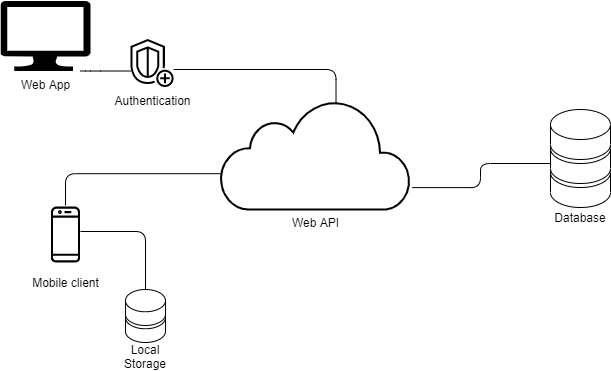
\includegraphics[scale=0.75]{images/Diagrama-do-projeto}
    \caption{Diagrama do projeto Queuality.}
    \label{fig:diagrama}
\end{figure}

\pagebreak
\section{Requisitos Funcionais}
\subsection{Base de Dados} \label{baseDeDadosReference}
Nesta secção é apresentada a proposta de solução para a base de dados utilizada. Esta estará responsável
por armazenar a informação da Web API. No projeto presente a base de dados é não relacional, neste caso do tipo
\textit{Document Store} utilizando a tecnologia \textit{MongoDB}\cite{mongoDBReference}. A escolha deste tipo de base de dados deu-se ao 
facto de ser algo não muito explorado no curso e algo bastante usado na indústria. Base de dados do tipo documento
tem também como vantagem guardar os dados de forma bastante similhante aos objetos usados na aplicação em questão, reduzindo 
assim a necessidade de haver tradução dos dados como estariam guardados numa base de dados relacional para os dados que a aplicação recebe.
Na figura \ref{fig:figure1} encontra-se o modelo de dados utilizado neste projeto. Foi com base neste modelo que se criou as coleções e campos necessários para poder 
guardar a informação necessária.\par
\begin{figure}[h]
    \centering
    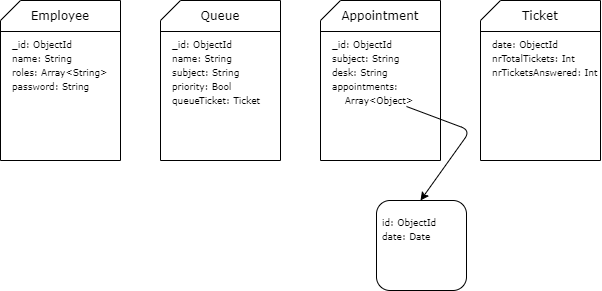
\includegraphics[scale=0.75]{Data-Model}
    \caption{Modelo de Dados do Queuality.}
    \label{fig:figure1}
\end{figure}
Começou-se por definir as coleções necessários para lidar com um sistema de gestão de senhas. Estas entidades ainda estão abertas para melhoramentos ou adição de campos
que se considerem necessários guardar. Assim, definiu-se a coleção \textit{Employee} \ref{fig:figure1} ilustrada na figura que irá conter a informação necessária para identificar um funcionário assim 
como os seus roles como funcionário da empresa em questão. Seguidamente, foi defenida a coleção \textit{Queue} ilustrada na figura \ref{fig:figure1} que irá conter o nome da fila, o assunto que irá ser tratado nessa fila
e também irá ser guardada a informação das senhas da fila em questão. A informação sobre as senhas de cada fila irá ser guardado num objecto definido por \textit{Ticket} em que irá conter o número de pessoas que foram atendidas
daquela fila, o número total de pessoas que tiraram senha naquela fila e finalmente a data que irá servir para reiniciar todos os dias a contagem das senhas a zero.
\subsection{Aplicação \textit{Web}}
Nesta secção é apresentada a proposta de solução para a aplicação \textit{web}. A aplicação web foi realizada com o propósito de ser utilizada pelos funcionários 
da empresa que usufruir do sistema em que irão ser englobadas diferentes ações a realizar, gerir as filas, gerir marcações realizadas e avançar nas senhas.
A aplicação irá ter um serviço de autenticação \textit{OpenId}\cite{openIDReference} para que apenas os funcionários autenticados possam realizar ditas ações.\par
Apesar de ainda não decidido, possivelmente os diferentes \textit{roles} que irão existir não poderão ter acesso a todos os links de navegação que 
irão estar disponíveis na aplicação \textit{web}.\par
Na aplicação escolheu-se usar a tecnologia \textit{React}\cite{reactReference} com \textit{TypeScript}\cite{typescriptReference}. A escolha de \textit{React}\cite{reactReference}
para \textit{frontend} sucedeu-se visto que é uma tecnologia cada vez mais usada na indústria, é bastante simples de compilar e fácil e apresenta qualidade na \textit{user interface} 
o que é bastante importante para quem usufruir da aplicação. Para a linguagem estava-se indeciso entre \textit{JavaScript}\cite{javascriptReference} ou \textit{TypeScript}\cite{typescriptReference} acabando-se por escolher a última visto que
usa tipos o que consegues corrigir erros que poderia facilmente acontecer em \textit{JavaScript}\cite{javascriptReference} que é uma linguagem fracamente tipificada.\par
Neste momento todos os funcionários autenticados irão ter acesso à aplicação toda.\par
Na figura \ref{fig:figure2} está presente o diagrama de navegação utilizado para definir as diferentes páginas que a aplicação irá conter.
\begin{landscape}
    \begin{figure}
        \centering
        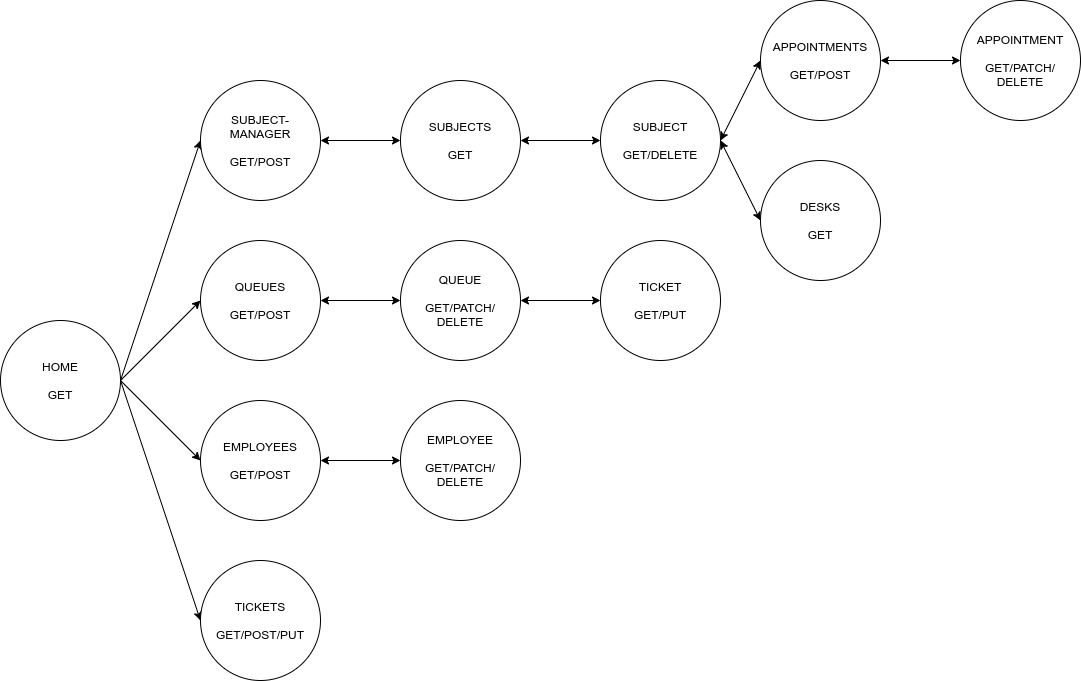
\includegraphics[scale=0.5]{Hypermedia-Navigation}
        \caption{Diagrama de navegação da Aplicação \textit{Web}}
        \label{fig:figure2}
    \end{figure}
\end{landscape} 
De seguida, desenhou-se a página de gestão das filas (Figura \ref{fig:figure3}) em serão apresentados o nome das filas, o assunto das filas, a prioridade e onde
será possível editar, apagar e adicionar filas. Estas ações apenas aos funcionários que o papel designado para tal.\par
\begin{figure}[h]
    \centering
    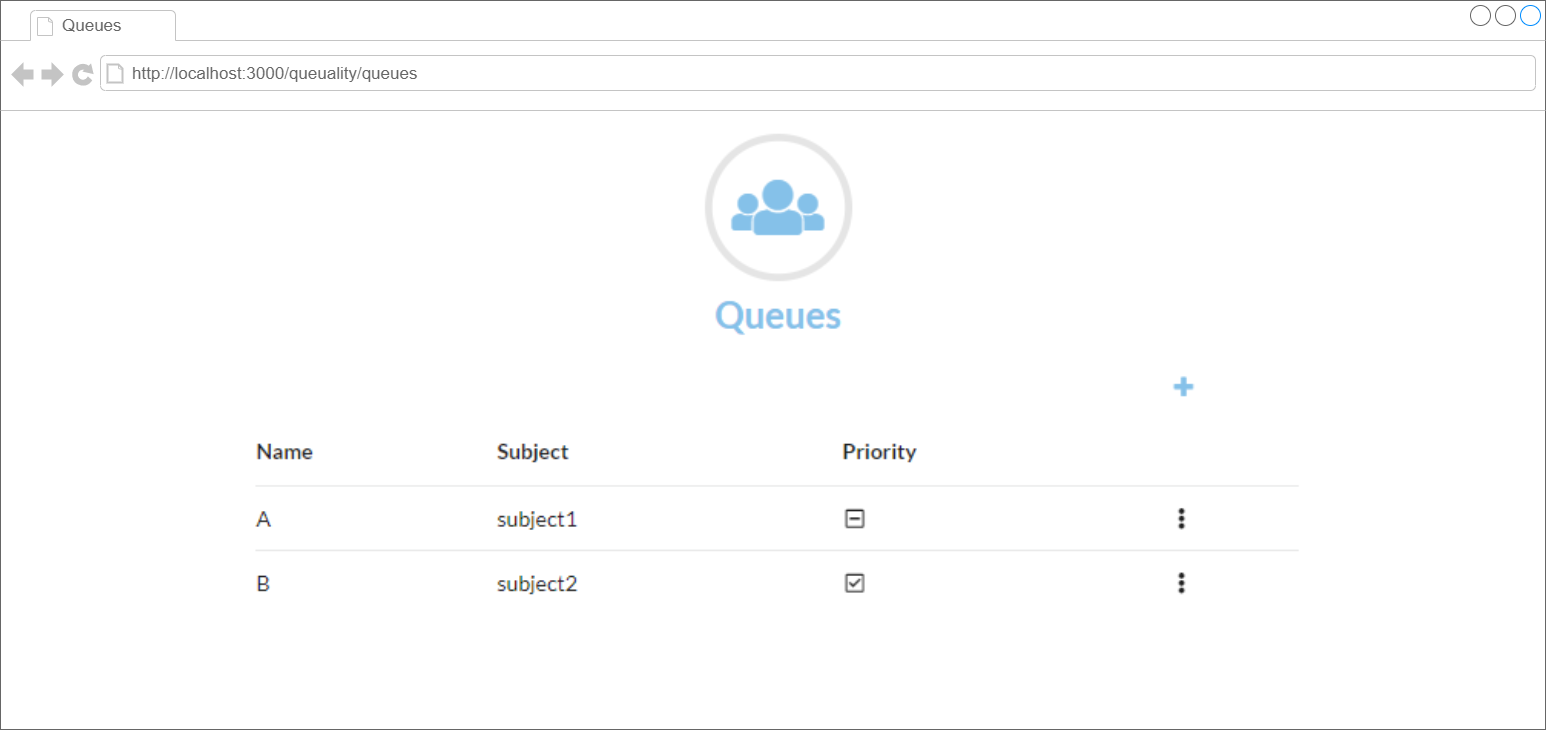
\includegraphics[scale=0.25]{QueuesMock}
    \caption{Mock da Aplicação \textit{Web}: Gestão das filas}
    \label{fig:figure3}
\end{figure}
Já na página dos tickets é possível visualizar as próximas cinco senhas a serem chamadas assim como o funcionário ter um botão em que lhe será possível avançar na
fila. Um \textit{mock} desta página encontra-se na figura (Figura \ref{fig:figure4}).
\begin{figure}[h]
    \centering
    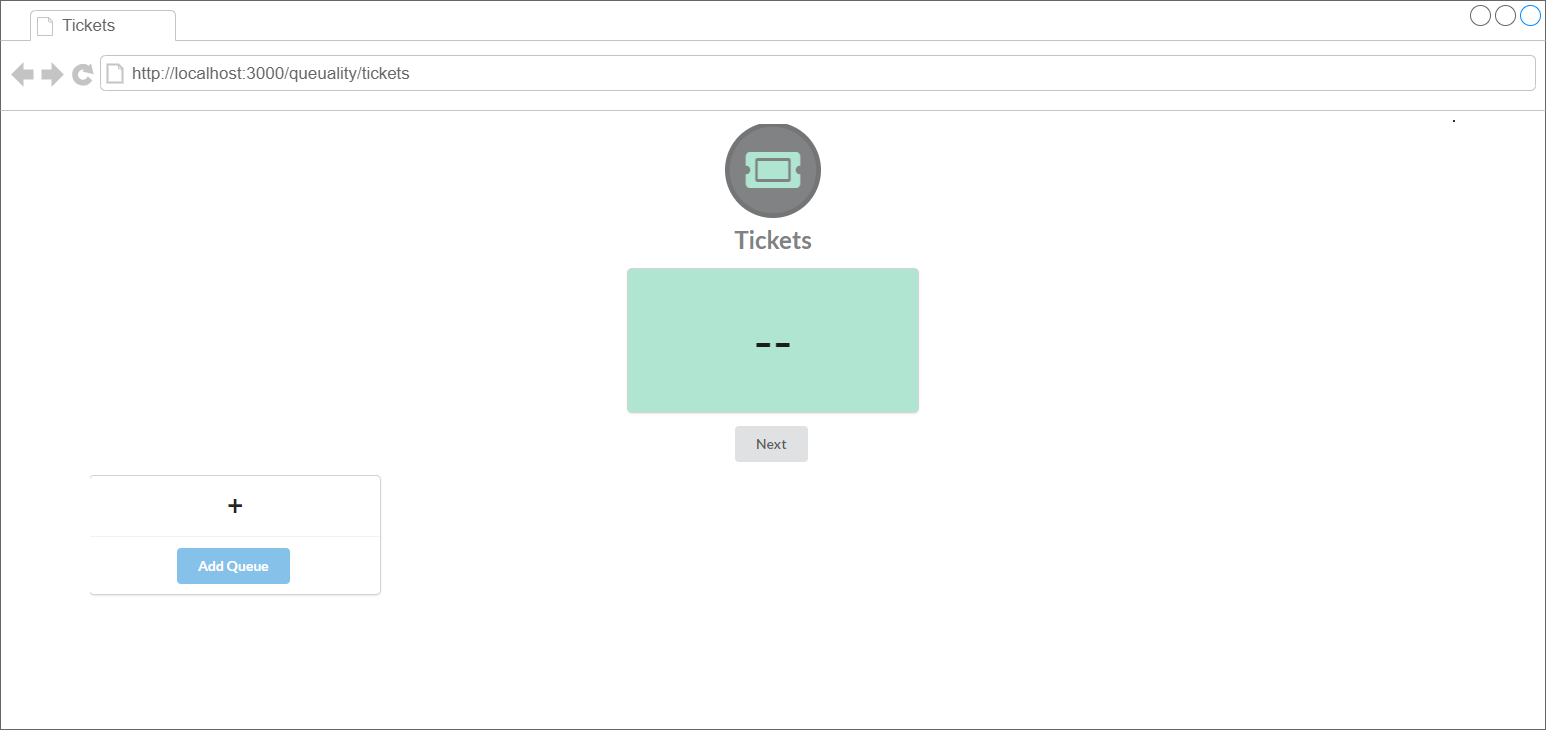
\includegraphics[scale=0.25]{TicketsMocks}
    \caption{Mock da Aplicação \textit{Web}: Gestão das senhas}
    \label{fig:figure4}
\end{figure}
\pagebreak
\subsection{\textit{Web API}}
Nesta secção é descrita a solução realizada neste projeto para a construção da \textit{Web API}. A \textit{API} foi escrita com recurso à linguagem \textit{JavaScript}\cite{javascriptReference}.
Esta linguagem é bastante utilizada no mundo de \textit{web development} devido à sua simplicidade de aprendizagem, semelhança com outras liguagens, 
compactação do código e velocidade de execução. No entanto, devido à não existência de um ambiente virtual de execução nativo da linguagem \textit{JavaScript}\cite{javascriptReference}
é necessário ainda a utilização de um ambiente de execução que possa tirar o maior partido da linguagem e facilite a execução da \textit{API} em \textit{background}
para tal foi utilizado o ambiente \textit{Node.js}\cite{nodeJsReference} para a execução da \textit{API}. As próximas subsecções explicam em detalhe os aspetos mais importantes da \textit{API}.

\subsubsection{Express}
O módulo Express\cite{expressReference} foi utilizado para a implementação da \textit{Web API}, visto existir uma maior confortabilidade com este módulo devido à sua
utilização na cadeira Programação na Internet. Este módulo é \textit{open-source}, por isso desenvolvido pela comunidade que utiliza \textit{Node.js}\cite{nodeJsReference}
como seu ambiente virtual de execução. Esta característica torna o módulo bastante completo pois quando a comunidade sente a necessidade de alguma funcionalidade
esta é implementada muito mais rapidamente, tornando também o modulo bastante versátil.

As principais vantagens da utilização deste módulo para além das descritas acima são ainda a facilidade de incorporação com outros módulos,
a criação automática de um servidor HTTP para as suas aplicações, livre-arbítrio nas diferentes decisões de arquitetura da aplicação e o suporte
integrado para a criação de uma \textit{REST API}.

\subsubsection{Acesso à Base de Dados}
Devido à escolha de MongoDB\cite{mongoDBReference} para o alojamento da base de dados como referido da secção \ref{baseDeDadosReference} optou-se também por utilizar o módulo desenvolvido pela mesma empresa, visto este apresentar 
um suporte e documentação mais completos para todas as funcionalidades disponibilizadas. Para a implementação deste acesso foi criado um módulo que
realiza a comunicação com a base de dados e outros quatro módulos que servem como repositórios para cada coleção. É através destes repositórios que 
são realizadas todas as verificações necessárias para as operações realizadas na \textit{API}. Existe ainda os módulos de serviço onde são implementadas
todas as funcionalidades da \textit{API} que necessitem de acesso à base de dados.

\subsubsection{Autenticação}
Tendo em atenção que o Queuality pretende ser um projeto que possa ser adotado por qualquer empresa optou-se por utilizar um sistema de autenticação
aberto seguindo o protocolo \textit{OpenID}\cite{openIDReference} em vez de ser criado um sistema de autenticação fechado. Desta forma qualquer empresa que adote o projeto
pode facilmente utilizar o seu sistema de autenticação para permitir aos seus trabalhadores acesso ao sistema de gestão de base de dados, acrescentando
apenas algumas variáveis de ambiente ao seu servidor.

Para efeitos de teste e demonstração foi escolhido o sistema de autenticação da Google, visto o grupo já ter tido experiência com este sistema na cadeira 
Segurança Informática.
\pagebreak
\subsection{Aplicação Móvel}
A aplicação móvel deste sistema foi desenvolvida em \textit{TypeScript}\cite{typescriptReference} juntamente com \textit{React}\cite{reactReference} 
com o auxílio da \textit{framework Ionic}\cite{ionicReference}. Esta foi escolhida sobre outras opções uma vez que é possível desenvolver uma aplicação \textit{Android}
e uma aplicação \textit{iOS} com o mesmo código. Outro ponto que nos fez escolher \textit{Ionic}\cite{ionicReference} em vez de \textit{React Native}\cite{reactNativeReference} foi o facto de \textit{Ionic}\cite{ionicReference}
pedir apenas conceitos básicos de \textit{React}\cite{reactReference} enquanto que \textit{React Native}\cite{reactNativeReference} pede conhecimentos avançados sobre o mesmo.\par
A aplicação móvel destina-se exclusivamente aos clientes da empresa utilizadora deste serviço. 
A aplicação desenvolvida divide-se em três módulos principais: O módulo de filas, o módulo de senhas
e o módulo de marcações, sendo estes separados por abas. A figura \ref{fig:diam} ilustra as funcionalidades presentes na aplicação móvel.\par
\begin{figure}[h]
    \centering
    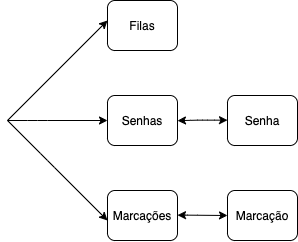
\includegraphics[width=0.25\textwidth]{DiagramaMobileApp}
    \caption{Diagrama de navegação da Aplicação Móvel}
    \label{fig:diam}
\end{figure}

A primeira página a ser desenvolvida foi a página do módulo das filas. O principal objetivo desta página é apresentar ao cliente
todas as filas existentes no sistema (nome, assunto e se é uma fila prioritária ou não), em que número vai cada fila e,
ao carregar numa fila, dar a possbilidade ao cliente de tirar uma senha para a mesma. Nas figuras \ref{fig:mockQueues} é possível observar 
\textit{mocks} da página de filas tanto para \textit{Android} como para \textit{iOS}.\par
\pagebreak
\begin{figure}[h]
\centering
\begin{subfigure}[h]{.5\textwidth}
  \centering
  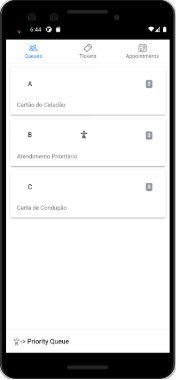
\includegraphics[scale=0.65]{mockQueuesAndroid}
  \caption{Android}
  \label{fig:queuesAndroid}
\end{subfigure}%
\begin{subfigure}[h]{.5\textwidth}
  \centering
  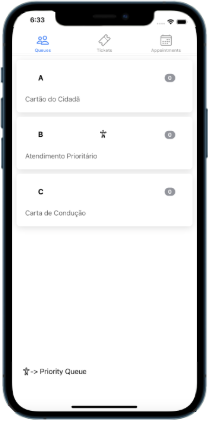
\includegraphics[scale=0.55]{mockQueuesIOS}
  \caption{iOS}
  \label{fig:queuesIos}
\end{subfigure}
\caption{Mock da página das filas}
\label{fig:mockQueues}
\end{figure}
Na página das senhas é apresentada ao cliente uma lista com as suas senhas (com um máximo de uma senha por fila) e, carregando na senha,
o cliente será redirecionado para outra página com os detalhes da mesma, entre as quais, o seu número, o assunto da fila, quantas pessoas
estão à sua frente e em que número vai a fila para a qual tirou senha. Terá também a possbilidade de cancelar a senha em ambas as páginas
deste módulo.\par

\begin{figure}
\vspace{-1 cm}
\centering
\begin{subfigure}[h]{0.5\textwidth}
  \centering
  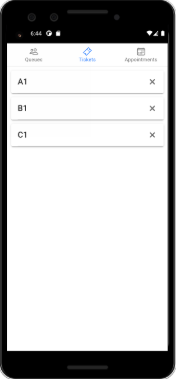
\includegraphics[scale=0.65]{mockTicketsAndroid}
  \caption{Android}
  \label{fig:ticketsAndroid}
\end{subfigure}%
\begin{subfigure}[h]{0.5\textwidth}
  \centering
  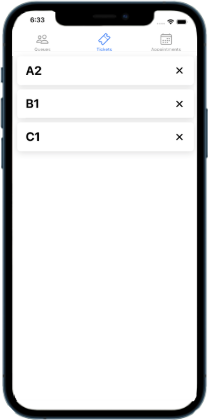
\includegraphics[scale=0.55]{mockTicketsIOS}
  \caption{iOS}
  \label{fig:ticketsIos}
\end{subfigure}
\caption{Mock da página das senhas}
\label{fig:mockTickets}
\end{figure}

\begin{figure}
\centering
\begin{subfigure}[h]{0.5\textwidth}
  \centering
  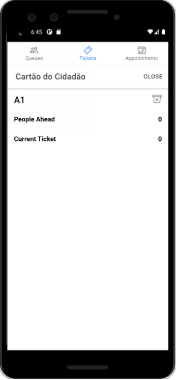
\includegraphics[scale=0.65]{mockTicketDetailsAndroid}
  \caption{Android}
  \label{fig:ticketDetailsAndroid}
\end{subfigure}%
\begin{subfigure}[h]{0.5\textwidth}
  \centering
  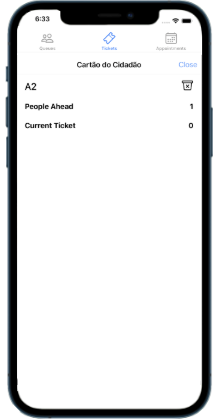
\includegraphics[scale=0.55]{mockTicketDetailsIOS}
  \caption{iOS}
  \label{fig:ticketDetailsIos}
\end{subfigure}
\caption{Mock da página dos detalhes de uma senha}
\label{fig:mockTicketDetails}
\end{figure}

\pagebreak
\section{Requisitos Não Funcionais}
Para a solução deste projeto os recursos serão alocados numa base de dados não relacional, para dar
oportunidade ao aprofundamento dos conhecimentos sobre a mesma. Esta base de dados irá guardar os
utilizadores autenticados e as suas respetivas funções. Cada utilizador anónimo terá uma base de dados
local que guardará marcações e/ou senhas juntamente com a informação adicional que for necessária
no decorrer do projeto.
Tenciona-se realizar \textit{deployment} na \textit{cloud} de modo que o projeto tenha oportunidade de ser
distribuído a potenciais interessados. Terá a possibilidade de receber relatórios de análise de forma a
ser possível monitorizar os potenciais problemas que possam vir a ocorrer no sistema.
\pagebreak
\section{Estado atual do Projeto}
Neste momento, a componente servidora e a base de dados encontram-se implementadas, no entanto sempre prontas para melhoramentos. 
Em relação ao \textit{frontend}, na aplicação móvel, a atividade das filas encontra-se completa e a de o utilizador poder tirar uma senha 
também, ficando a faltar na sua totalidade as atividade das marcações. Em relação a aplicação web falta implementar a parte da autenticação,
a página da informação dos funcionários e a das marcações. Encontra-se completamente implementada a página das filas e a página das senhas 
encontra-se parcialmente implementada faltando apenas tomar algumas decisões finais.

\pagebreak
\begin{thebibliography}{9}    
    \bibitem{mongoDBReference} 
    MongoDB,\\\texttt{https://www.mongodb.com/}.
    Consultado a 15/04/2021
    \bibitem{reactReference} 
    \textit{React},\\\texttt{https://reactjs.org/}.
    Consultado a 20/04/2021    
    \bibitem{typescriptReference} 
    TypeScript,\\\texttt{https://www.typescriptlang.org/}.
    Consultado a 20/04/2021
    \bibitem{javascriptReference}
    JavaScript,\\\texttt{https://www.typescriptlang.org/}.
    Consultado a 12/04/2021
    \bibitem{ionicReference}
    Ionic, \\\texttt{https://ionicframework.com/}.
    Consultado a 06/06/2021
    \bibitem{reactNativeReference}
    React Native \\\texttt{https://reactnative.dev/}.
    Consultado a 12/04/2021
    \bibitem{openIDReference}
    OpenID, \\\texttt{https://openid.net/}.
    Consultado a 23/05/2021
    \bibitem{nodeJsReference}
    NodeJs, \\\texttt{https://nodejs.org/}.
    Consultado a 02/04/2021
    \bibitem{expressReference}
    Express, \\\texttt{https://expressjs.com/}.
    Consultado a 02/04/2021
\end{thebibliography}

\pagebreak
\appendix
\section{Documentação das Rotas da API}
O URL base desta API é /api. As próximas secções irão descrever cada endpoint da API.

\subsection{Módulo de Filas}
O Módulo de Filas contem 3 rotas distintas às quais são feitos 5 pedidos diferentes. Nos próximos pontos 
iremos descrever cada um desses pedidos
\subsubsection{GET /queues}
Este pedido retorna a lista das filas existentes em sistema. Tanto o administrador como os clientes deste sistema tem acesso a este pedido.\par
\vspace{0.5 cm}
 \textbf{Pedido}\par
Headers: content-type: aplication/json\par
\vspace{0.5 cm}
\textbf{Resposta}\par

Status Code: 200\par
Headers: content-type: aplication/json\par
Body: 
\begin{minted}{json}

{    
    "class": ["Queues"],
    "properties": [        
        {             
            "_id": "60b3e2830e97c070513f24a6",
            "name": "A",
            "priority": false,
            "queueTicket": {                 
                "nrTicketsAnswered": 0,                 
                "nrTotalTickets": 1,                 
                "date": "Sun Jun 13 2021"             
            },
            "subject": "Cartão do Cidadão"         
        },
        {             
            "_id": "60b3e2f20e97c070513f2512",             
            "name": "B",
            "priority": true,
            "queueTicket": {
                "nrTicketsAnswered": 0,                 
                "nrTotalTickets": 1,
                "date": "Sun Jun 13 2021"             
            },
            "subject": "Atendimento Prioritário"
        },
        {
            "_id": "60bbf1490fa7216722109854",
            "name": "C",
            "priority": false,
            "queueTicket": {
                "nrTicketsAnswered": 0,
                "nrTotalTickets": 1,
                "date": "Sun Jun 13 2021"
            },
            "subject": "Carta de Condução"
        }     
    ],    
    "entities": [                      
        {
            "rel": ["/rel/queue"],
            "properties": {
                "_id": "60b3e2830e97c070513f24a6",                     
                "name": "A",
                "priority": false,
                "queueTicket": {
                    "nrTicketsAnswered": 0,                        
		    "nrTotalTickets": 1,
                    "date": "Sun Jun 13 2021"                     
                },                     
                "subject": "Cartão do Cidadão"                
            },
            "class": ["Queue"],
            "links": [
                {
                    "rel": ["self"],
                    "href": "/api/queues/60b3e2830e97c070513f24a6"      
                },
                {
                    "rel": ["/rel/current-ticket"],                       
                    "href":"/api/queues/60b3e2830e97c070513f24a6/current-ticket"
                }                 
            ],
            "actions": [                     
                {                         
                    "name": "update-queue",
                    "title": "Update a Queue",
                    "method": "PATCH",
                    "href": "/api/queues/60b3e2830e97c070513f24a6",
                    "type": "application/vnd.siren+json",
                    "fields": [                             
                        {
                            "name": "priority",                               
                            "type": "boolean"                            
                        },                             
                        {
                            "name": "subject",                                
                            "type": "text"                             
                        }                         
                    ]                     
                },
                {
                    "name": "delete-queue",
                    "title": "Delete a Queue",
                    "method": "DELETE",
                    "href": "/api/queues/60b3e2830e97c070513f24a6",
                    "type": "application/vnd.siren+json"                     
                }                 
            ],
            "title": "Get Queue"
        },
        {
            "rel": ["/rel/queue"],
            "properties": {
                "_id": "60b3e2f20e97c070513f2512",
                "name": "B",
                "priority": true,
                "queueTicket": {
                    "nrTicketsAnswered": 0,                         
                    "nrTotalTickets": 1,
                    "date": "Sun Jun 13 2021"                     
                },
                "subject": "Atendimento Prioritário"
            },
            "class": ["Queue"],                 
            "links": [
                {
                    "rel": ["self"],
                    "href": "/api/queues/60b3e2f20e97c070513f2512"          
                },                     
                {                         
                    "rel": ["/rel/current-ticket"],                       
                    "href":"/api/queues/60b3e2f20e97c070513f2512/current-ticket"
                }                 
            ],
            "actions": [
                {
                    "name": "update-queue",
                    "title": "Update a Queue",
                    "method": "PATCH",
                    "href": "/api/queues/60b3e2f20e97c070513f2512",
                    "type": "application/vnd.siren+json",
                    "fields": [                             
                        {
                            "name": "priority",
                            "type": "boolean"
                        },              
                        {
                            "name": "subject",                                
                            "type": "text"
                        }                         
                    ]                     
                },                     
                {
                    "name": "delete-queue",
                    "title": "Delete a Queue",
                    "method": "DELETE",
                    "href": "/api/queues/60b3e2f20e97c070513f2512",
                    "type": "application/vnd.siren+json"                     
                }                 
            ],
            "title": "Get Queue"             
        },
        {
            "rel": ["/rel/queue"],
            "properties": {                     
                "_id": "60bbf1490fa7216722109854",
                "name": "C",
                "priority": false,
                "queueTicket": {
                    "nrTicketsAnswered": 0,                         
                    "nrTotalTickets": 1,
                    "date": "Sun Jun 13 2021"
                },
                "subject": "Carta de Condução"                 
            },
            "class": ["Queue"],
            "links": [                     
                {                         
                    "rel": ["self"],
                    "href": "/api/queues/60bbf1490fa7216722109854"        
                },
                {
                    "rel": ["/rel/current-ticket"],                         
                    "href":"/api/queues/60bbf1490fa7216722109854/current-ticket"
                }
            ],
            "actions": [
                {
                    "name": "update-queue",
                    "title": "Update a Queue",
                    "method": "PATCH",
                    "href": "/api/queues/60b3e2f20e97c070513f2512",
                    "type": "application/vnd.siren+json",
                    "fields": [                             
                        {
                            "name": "priority",
                            "type": "boolean"
                        },              
                        {
                            "name": "subject",                                
                            "type": "text"
                        }                         
                    ]                     
                },                     
                {
                    "name": "delete-queue",
                    "title": "Delete a Queue",
                    "method": "DELETE",
                    "href": "/api/queues/60b3e2f20e97c070513f2512",
                    "type": "application/vnd.siren+json"                     
                }                 
            ],
            "title": "Get Queue"
        }
    ],
    "links": [
        {             
            "rel": ["self"],
            "href": "/api/queues"
        }     
    ],
    "actions": [
        {
            "name": "add-queue",
            "title": "Add a Queue",
            "method": "POST",
            "href": "/api/queues",
            "type": "application/vnd.siren+json",
            "fields": [
                {
                    "name": "name",
                    "type": "text"
                },
                {
                    "name": "priority",
                    "type": "boolean"
                },
                {
                    "name": "subject",
                    "type": "text"
                }                
            ]             
        }
    ] 
}
\end{minted}
\pagebreak
\subsubsection{POST /queues}
Este pedido adiciona uma fila ao sistema. Apenas o administrador tem acesso a este pedido.\par
\vspace{0.5 cm}
\textbf{Pedido}

Headers: content-type: aplication/json\par
Body:
\begin{minted}{json}
{
    "name": "C",
    "priority": false,
    "subject": "Carta de Condução"
}
\end{minted}


  \textbf{Resposta}\par
Status Code : 201 \par
Headers : content-type: aplication/json \par
Body:
\begin{minted}{json}
 {
    "class": ["Queue"],
    "properties": {
        "_id": "60c655d50fa72167221187b0",
        "name": "C",
        "priority": false,
        "queueTicket": {
            "nrTotalTickets": 0,
            "nrTicketsAnswered": 0,
            "date": "Sun Jun 13 2021"         
        },
        "subject": "Carta de Condução"     
    },
    "entities": [],
    "links": [
        {
            "rel": ["self"],
            "href": "/api/queues"         
        }
    ],
    "actions": []
}
\end{minted}
\pagebreak
\subsubsection{PATCH /queues/:queueId}
Este pedido edita o assunto e/ou a prioridade de uma fila do sistema. Apenas o administrador tem acesso a este pedido.\par
\vspace{0.5 cm}
\textbf{Pedido}\par
Headers: content-type: aplication/json\par
Path Parameter : queueId - o identificador da fila\par
Body:
\begin{minted}{json}
{
    "subject": "finanças",
    "priority": true
}
\end{minted}



\textbf{Resposta}\par
Status Code: 200\par
Headers: content-type: aplication/json\par
Body:
\begin{minted}{json}
{     
    "class": ["Queue"],
    "properties": {
        "id": "60c655d50fa72167221187b0",         
        "name": "C",
        "priority": true,
        "queueTicket": {
            "nrTotalTickets": 0,
            "nrTicketsAnswered": 0,
            "date": "Sun Jun 13 2021"         
        },
        "subject": "finanças"    
    },
    "entities": [],
    "links": [         
        {             
            "rel": ["self"],
            "href": "/api/queues/60c655d50fa72167221187b0"
        }     
    ],
    "actions": []
}
\end{minted}
 \pagebreak
\subsubsection{DELETE /queues/:queueId}
Este pedido apaga uma fila do sistema. Apenas o administrador tem acesso a este pedido.\par
\vspace{0.5 cm}
\textbf{Pedido}\par
Headers : content-type: aplication/json \par
\vspace{0.5 cm}
\textbf{Resposta}\par
Status Code : 200 \par
Headers : content-type: aplication/json \par
Body: 
\begin{minted}{json}
{
    "class": ["Queue"],
    "properties": {},
    "entities": [],
    "links": [         
        {
            "rel": ["self"],
            "href": "/api/queues/60c655d50fa72167221187b0"
        }    
    ],
    "actions": []
}
\end{minted}
\pagebreak
\subsubsection{PUT /queues/:queueId/current-ticket}
Este pedido incrementa o número de senhas atedidas de uma fila do sistema. Tanto o administrador como o funcionário têm acesso a este pedido.\par
\vspace{0.5 cm}
\textbf{Pedido}\par
Headers: content-type: aplication/json\par
\vspace{0.5 cm}
\textbf{Resposta}\par
Status Code: 200\par                                                         
Headers: content-type: aplication/json\par
Body :
\begin{minted}{json}
 {
    "class": ["Current Ticket"],
    "properties": "C1",
    "entities": [],
    "links": [         
        {
            "rel": ["self"],
            "href": "/api/queues/60c655d50fa72167221187b0/current-ticket"       
        }     
    ],
    "actions": []
}     
\end{minted}
\pagebreak

\subsection{Módulo de Senhas}
O Módulo de Senhas contem 2 rotas distintas às quais são feitos 4 pedidos diferentes. Nos próximos pontos 
iremos descrever cada um desses pedidos
\subsubsection{GET /tickets/waiting-tickets}
Este pedido retorna o número de senhas em espera. Tanto o administrador como os funcionários deste sistema tem acesso a este pedido.\par
\vspace{0.5 cm}
 \textbf{Pedido}\par
Headers: content-type: aplication/json\par
\vspace{0.5 cm}
\textbf{Resposta}\par
Status Code: 200 \par                           
Headers: content-type: aplication/json\par 
Body: 
\begin{minted}{json}
{
    "class": ["Tickets"],
    "properties": 1,
    "entities": [],
    "links": [         
        {
            "rel": ["self"],
            "href": "/api/tickets/waiting-tickets"
        }
    ],
    "actions": []
}
\end{minted}
\pagebreak
\subsubsection{GET /tickets}
Este pedido retorna a lista de senhas em espera. Tanto o administrador como os funcionários deste sistema tem acesso a este pedido.\par
\vspace{0.5 cm}
 \textbf{Pedido}\par
Headers: content-type: aplication/json\par
\vspace{0.5 cm}
\textbf{Resposta}\par
Status Code: 200\par
Headers: content-type: aplication/json\par
Body: 
\begin{minted}{json}
{
    "class": ["Tickets"],
    "properties": [
        {
            "_id": "60b3e2830e97c070513f24a6",
            "ticketNumber": "A2",
            "subject": "Cartão do Cidadão",
            "priority": false         
        },
    ],
    "entities": [],
    "links": [         
        {
            "rel": ["self"],
            "href": "/api/tickets"         
        },        
        {           
            "rel": ["ticket-queues"],
            "href": "/api/queues"         
        }    
    ],
    "actions": [    
        {
            "name": "add-ticket",
            "title": "Add a Ticket",
            "method": "POST",
            "href": "/api/tickets",
            "type": "application/vnd.siren+json",
            "fields": [
                {
                    "name": "queueId",
                    "type": "text"
                }                
            ]
        },             
        {                 
            "name": "delete-ticket",
            "title": "Delete a Ticket",
            "method": "PUT",
            "href": "/api/tickets",
            "type": "application/vnd.siren+json"
        }    
    ]
}
\end{minted}
\pagebreak
\subsubsection{POST /tickets}
Este pedido adiciona uma senha à lista de espera. Apenas os clientes deste sistema têm acesso a este pedido.\par
\vspace{0.5 cm}
 \textbf{Pedido}\par
 Headers: content-type: aplication/json\par
Body:
 \begin{minted}{json}
 {
     "queueId": "60b3e2830e97c070513f24a6"
}     
 \end{minted}
 
 
\textbf{Resposta}\par
Status Code: 200\par 
Headers: content-type: aplication/json\par 
Body: 
\begin{minted}{json}
{
    "class": ["Tickets"],
    "properties": "A2",
    "entities": [],
    "links": [         
        {
            "rel": ["self"],
            "href": "/api/tickets"
        }
    ],
    "actions": []
}
\end{minted}
\pagebreak
\subsubsection{PUT /tickets}
Este pedido remove uma senha da lista de espera. Apenas os clientes deste sistema têm acesso a este pedido.\par
\vspace{0.5 cm}
\textbf{Pedido}\par
Headers: content-type: aplication/json\par
Body:
\begin{minted}{json}
{
    "ticket": "A1"
}
\end{minted}
    
\textbf{Resposta}\par
Status Code: 200\par 
Headers: content-type: aplication/json\par 
Body : 
\begin{minted}{json}
{
    "class": ["Tickets"],
    "properties": {},
    "entities": [],
    "links": [
        {
            "rel": ["self"],
            "href": "/api/tickets"
        }     
    ],
    "actions": []
}
\end{minted}
\pagebreak
\subsection{Módulo de Funcionários}
O Módulo de Funcionários contem 2 rotas distintas às quais são feitos 5 pedidos diferentes. Nos próximos pontos 
iremos descrever cada um desses pedidos
\subsubsection{GET /employees}
Este pedido retorna a lista dos funcionários. Apenas o administrador tem acesso a este pedido.\par
\vspace{0.5 cm}
\textbf{Pedido}\par
Headers: content-type: aplication/json
\vspace{0.5 cm}

\textbf{Resposta}\par

Status Code: 200\par
Headers: content-type: aplication/json\par
Body: 
\begin{minted}{json}
{
    "class": ["Employees"],
    "properties": [         
        {
            "_id": "60941a400e97c070512c05cd",
            "name": "Nome",
            "password":"$2b$10$Js0Kck5FqJjz0curcH36x.CUIhTzLM280/S/yL.2lRrJfOS4rXG/i",
            "roles":["admin"]
        },
        {
            "_id": "609421240e97c070512c069a",
            "name": "Nome2",
            "password":"$2b$10$EoK66j5LuYmUjSh4sQNb5OOS/uroG12/UXv6mWiR6rTR9hRyxSDLO",
            "roles": ["func"]         
        }
    ],
    "entities": [            
        {
            "rel": ["/rel/employee"],
            "properties": {},
            "class": ["Employee"],
            "links": [
                {
                    "rel": ["self"],
                    "href": "/api/employees/60941a400e97c070512c05cd"           
                }                 
            ],
            "actions": [],
            "title": ""             
        },
        {
            "rel": ["/rel/employee"],
            "properties": {},
            "class": ["Employee"],
            "links": [
                {
                    "rel": ["self"],
                    "href": "/api/queues/609421240e97c070512c069a"
                }                 
            ],
            "actions": [],
            "title": ""             
        }
    ],
    "links": [         
        {
            "rel": ["self"],
            "href": "/api/employees"
        }
    ],
    "actions": [             
        {
            "name": "add-employee",
            "title": "Add a Employee",
            "method": "POST",
            "href": "/api/employees",
            "type": "application/vnd.siren+json",
            "fields": [
                {
                    "name": "name",
                    "type": "text"
                },
                {
                    "name": "roles",
                    "type": "object"
                }                 
            ]             
        }     
    ]
}
\end{minted}
\pagebreak
\subsubsection{POST /employees}
Este pedido retorna a adiciona um funcionário. Apenas o administrador tem acesso a este pedido.\par
\vspace{0.5 cm}
\textbf{Pedido}\par
Headers: content-type: aplication/json\par  
Body: 
\begin{minted}{json}
{
    "name": "Nome3",
    "password" : "password",
    "roles": ["admin"]
}
\end{minted}


\textbf{Resposta}\par
Status Code: 201\par
Headers: content-type: aplication/json\par
Body: 
\begin{minted}{json}
{
    "class": ["Employees"],
    "properties": { 
        "_id": "60c671090fa72167221189a4",
        "name": "Nome3",
        "roles": ["admin"]    
    },
    "entities": [],
    "links": [
        {
            "rel": [ "self"],
            "href": "/api/employees"         
        },        
        {
            "rel": ["/rel/employee"],
            "href": "/api/employees/60c671090fa72167221189a4"
        }
    ],
    "actions": [] 
}
\end{minted}
\pagebreak
\subsubsection{GET /employees/:employeeId}
Este pedido retorna o funcionário com o identificador especificado no parametro do url. Apenas o administrador tem acesso a este pedido.\par
\vspace{0.5 cm}
\textbf{Pedido}\par
Headers: content-type: aplication/json\par
Path Parameter: employeeId- o identifacor do funcionário\par
\vspace{0.5 cm}
\textbf{Resposta}\par
Status Code: 200\par
Headers: content-type: aplication/json\par 
Body:
\begin{minted}{json}
{
    "class": ["Employee"],
    "properties": {
        "_id": "609421240e97c070512c069a",
        "name": "Nome",
        "roles": ["func"]     
    },
    "entities": [],
    "links": [
        {       
            "rel": ["self"],
            "href": "/api/employees/609421240e97c070512c069a"
        }     
    ],
    "actions": [
        {
            "name": "update-employee",
            "title": "Update an Employee",
            "method": "PATCH",
            "href": "/api/employees/609421240e97c070512c069a",
            "type": "application/vnd.siren+json",
            "fields": [                     
                {
                    "name": "roles",
                    "type": "object"                    
                }                 
            ]             
        },             
        {                
            "name": "delete-employee",
            "title": "Delete an Employee",
            "method": "DELETE",
            "href": "/api/employees/undefined",
            "type": "application/vnd.siren+json"             
        }    
    ]
}
\end{minted}
\pagebreak

\subsubsection{PATCH /employees/:employeeId}
Este pedido edita a password e/ou as funções do funcionário com o identificador especificado no parametro do url. Apenas o administrador tem acesso a este pedido.\par
\vspace{0.5 cm}
\textbf{Pedido}\par
Headers: content-type: aplication/json \par
Path Parameter: employeeId- o identifacor do funcionário \par
Body: 
\begin{minted}{json}
{
    "oldPassword": "password",
    "newPassword" : "pass",
    "roles": ["func"]
}
\end{minted}

\textbf{Resposta}\par
Status Code: 200\par
Headers: content-type: aplication/json\par 
Body: 
\begin{minted}{json}
{
    "class": ["Employee"],
    "properties": {},
    "entities": [],
    "links": [         
        {
            "rel": ["self"],
            "href": "/api/employees/609421240e97c070512c069a"
        },
        {
            "rel": [ "/rel/employees"],
            "href": "/api/employees"
        }
    ],
    "actions": []
}
\end{minted}
\pagebreak
\subsubsection{DELETE /employees/:employeeId}
Este pedido apaga o funcionário com o identificador especificado no parametro do url. Apenas o administrador tem acesso a este pedido.\par
\vspace{0.5 cm}
\textbf{Pedido}\par
Headers: content-type: aplication/json \par
Path Parameter: employeeId- o identifacor do funcionário \par
\vspace{0.5 cm}
\textbf{Resposta}\par
Status Code: 200\par
Headers: content-type: aplication/json\par 
Body: 
\begin{minted}{json}
{
    "class": ["Employee"],
    "properties": {},
    "entities": [],
    "links": [         
        {
            "rel": [ "/rel/employees"],
            "href": "/api/employees"
        }
    ],
    "actions": []
}
\end{minted}

\end{document}